\begin{figure*}[t!]
\begin{centering}
	\begin{subfigure}[b]{0.85\textwidth}
                \centering
		\caption{Timeline}
                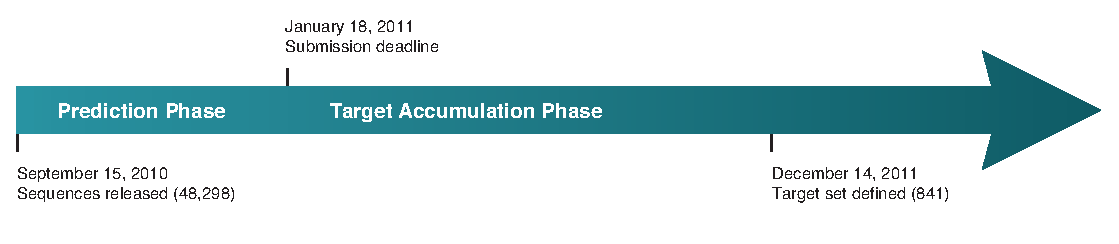
\includegraphics[width=\textwidth]{Figures/intro/NM_1A}
                \label{fig:cafa1}
        \end{subfigure}%

	\begin{subfigure}[b]{0.55\textwidth}
                \centering
                \caption{Target counts}                
                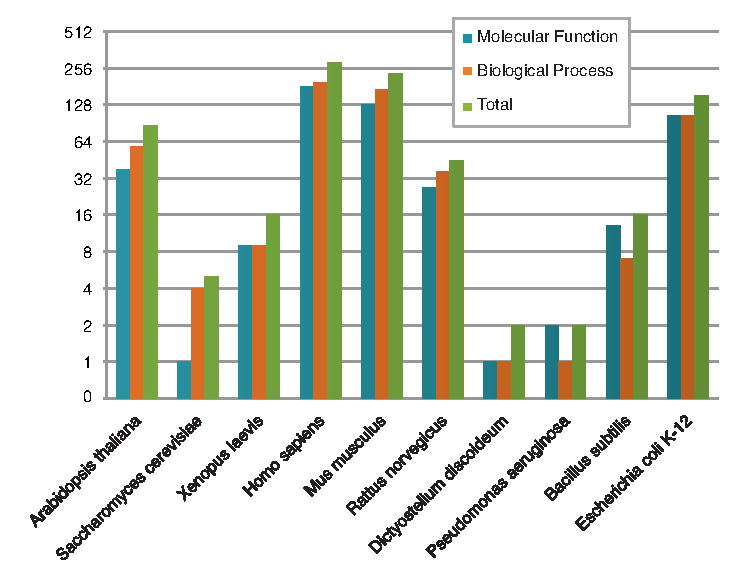
\includegraphics[width=\textwidth]{Figures/intro/NM_1B}
                \label{fig:cafa2}
        \end{subfigure}
	\quad
	\begin{subfigure}[b]{0.30\textwidth}
                \centering
                \caption{Functional terms}                
                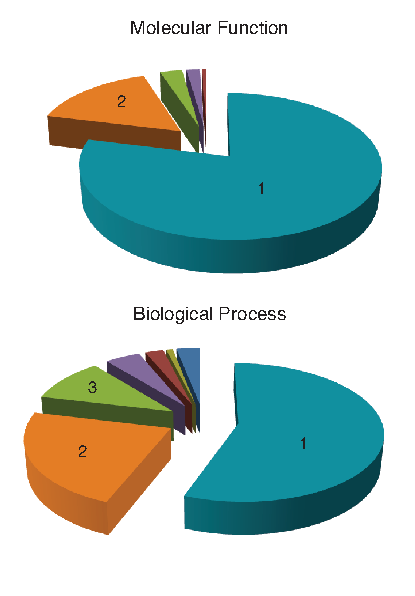
\includegraphics[width=\textwidth]{Figures/intro/NM_1C}
                \label{fig:cafa3}
        \end{subfigure}%

\end{centering}
\caption[CAFA Experiment and data]{\Cref{fig:cafa1}: Timeline for the CAFA experiment. \Cref{fig:cafa2}: Number of target sequences per organism. The graph shows the number of target sequences for each of the ontologies (Molecular Function and Biological Process) as well as the total number of targets, obtained as a union between sequences in the two ontologies. Of 866 proteins, 531 had Molecular Function annotations and 587 had Biological Process annotations. \Cref{fig:cafa3}: Distribution of target sequences in each ontology according to the number of leaf terms available for each protein sequence. For example, in the Molecular Function category, $79\%$ of proteins had one leaf term, $16\%$ had two leaf terms, and so on. A term is considered a leaf term for a particular target if no other GO term associated with that sequence is its descendant.}
\label{fig:SCOP_ROC}
\end{figure*}



